\Section{OS Concepts}


\begin{frame}{OS Concepts}

	We've talked about running instructions within a program

	But how do we get to that point?

	Before we can run the program, we need to boot the computer

	We generally also want to fire up an operating system

	The OS handles:

	\begin{itemize}
		\item memory allocation
		\item CPU time allocation
		\item device interfaces
		\item context switching (computer can juggle multiple tasks)
	\end{itemize}
\end{frame}

\Subsection{Booting}

\begin{frame}{Starting the Boot}
	\begin{itemize}
		\item As soon as we start executing an instruction, we are already fetching the next one
		\item But how do we know where to start?
		\item The location of the "boot block" is hard-coded. Often 0x00000000
		\item This is firmware. Non-volatile memory (aka users are not allowed to modify it)
	\end{itemize}
\end{frame}

\begin{frame}{Placeholder}
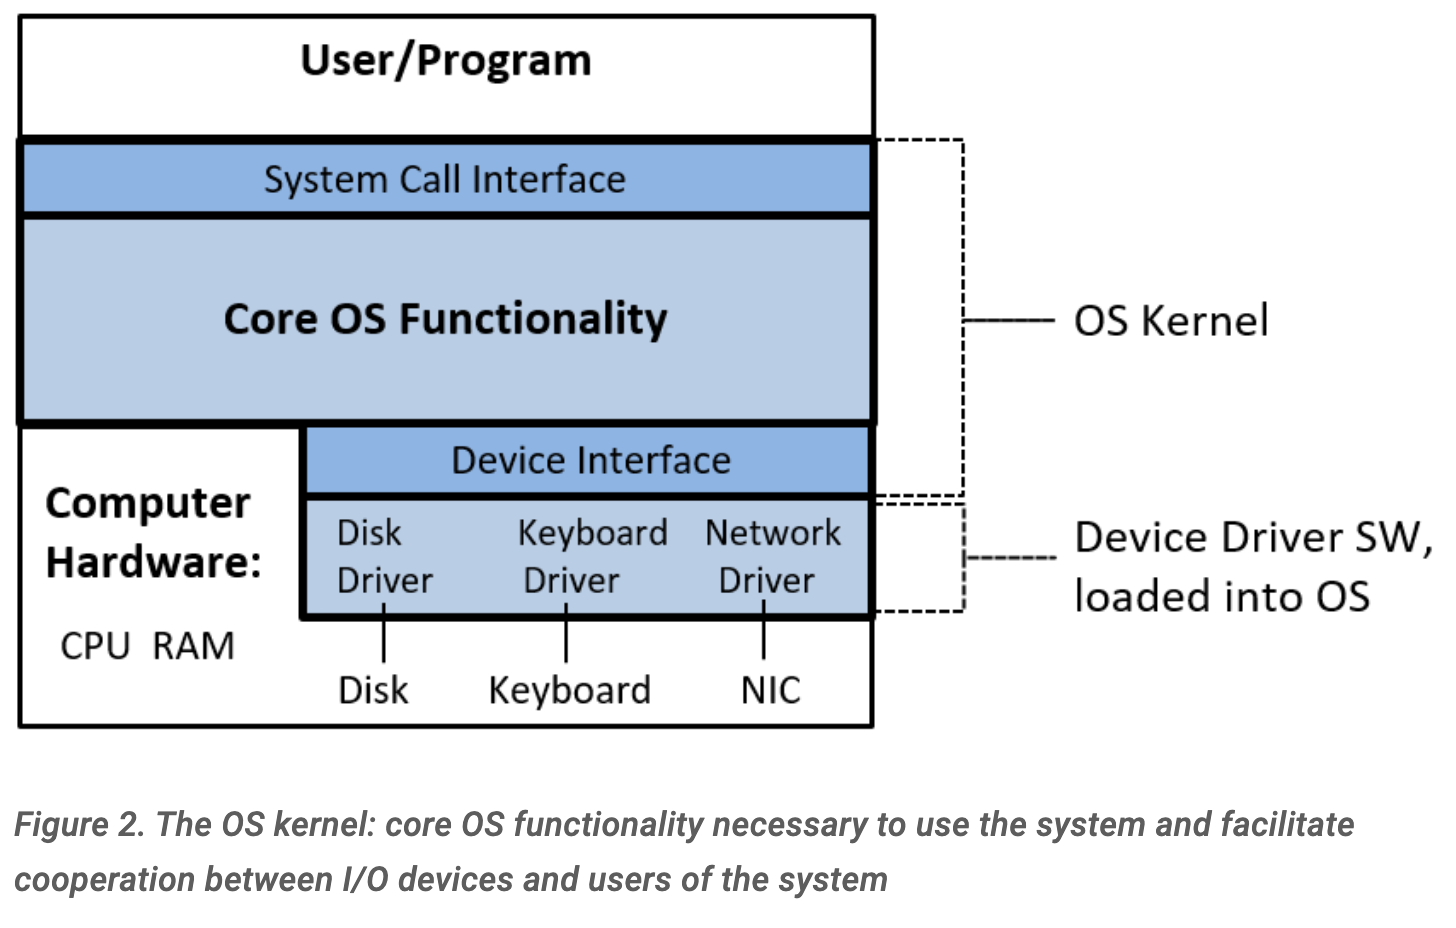
\includegraphics[width=\columnwidth]{images/device-drivers}
\end{frame}


\begin{frame}{Placeholder}
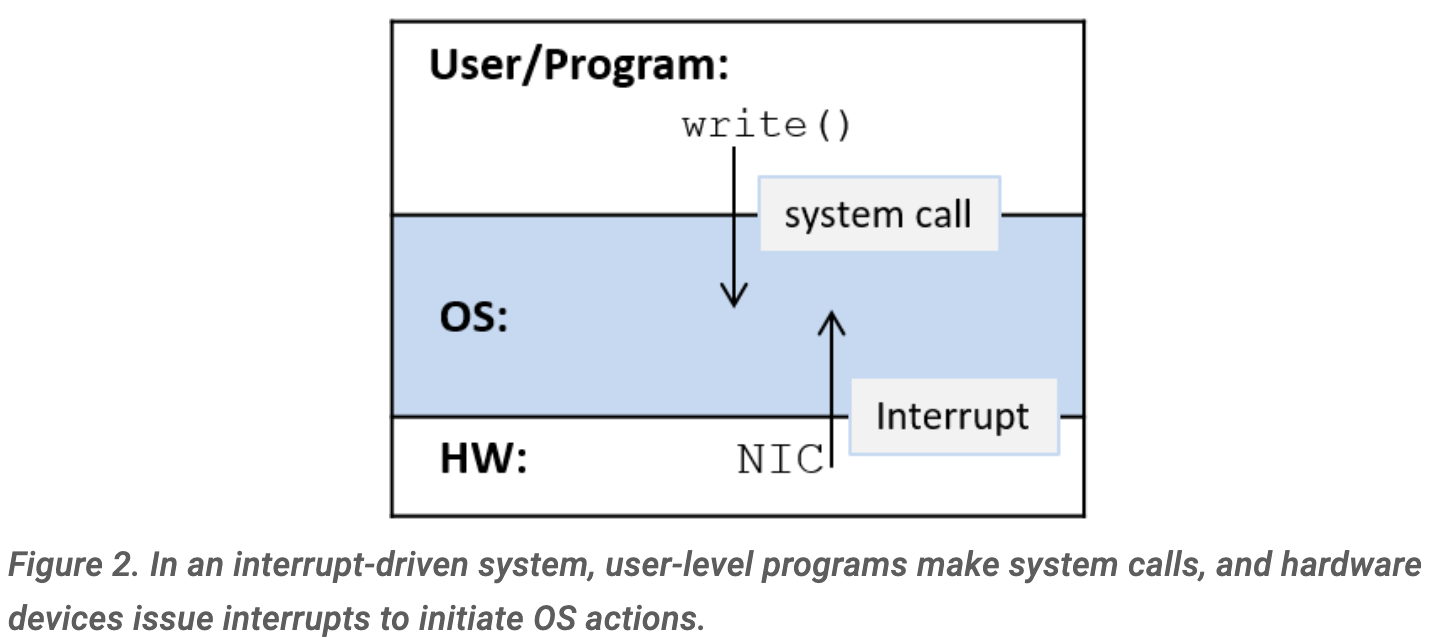
\includegraphics[width=\columnwidth]{images/call-to-os}
\end{frame}


\begin{frame}{Placeholder}
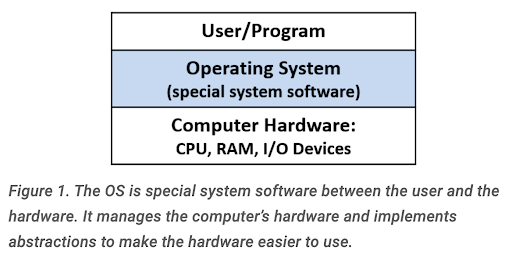
\includegraphics[width=\columnwidth]{images/os-location}
\end{frame}


\begin{frame}{Placeholder}
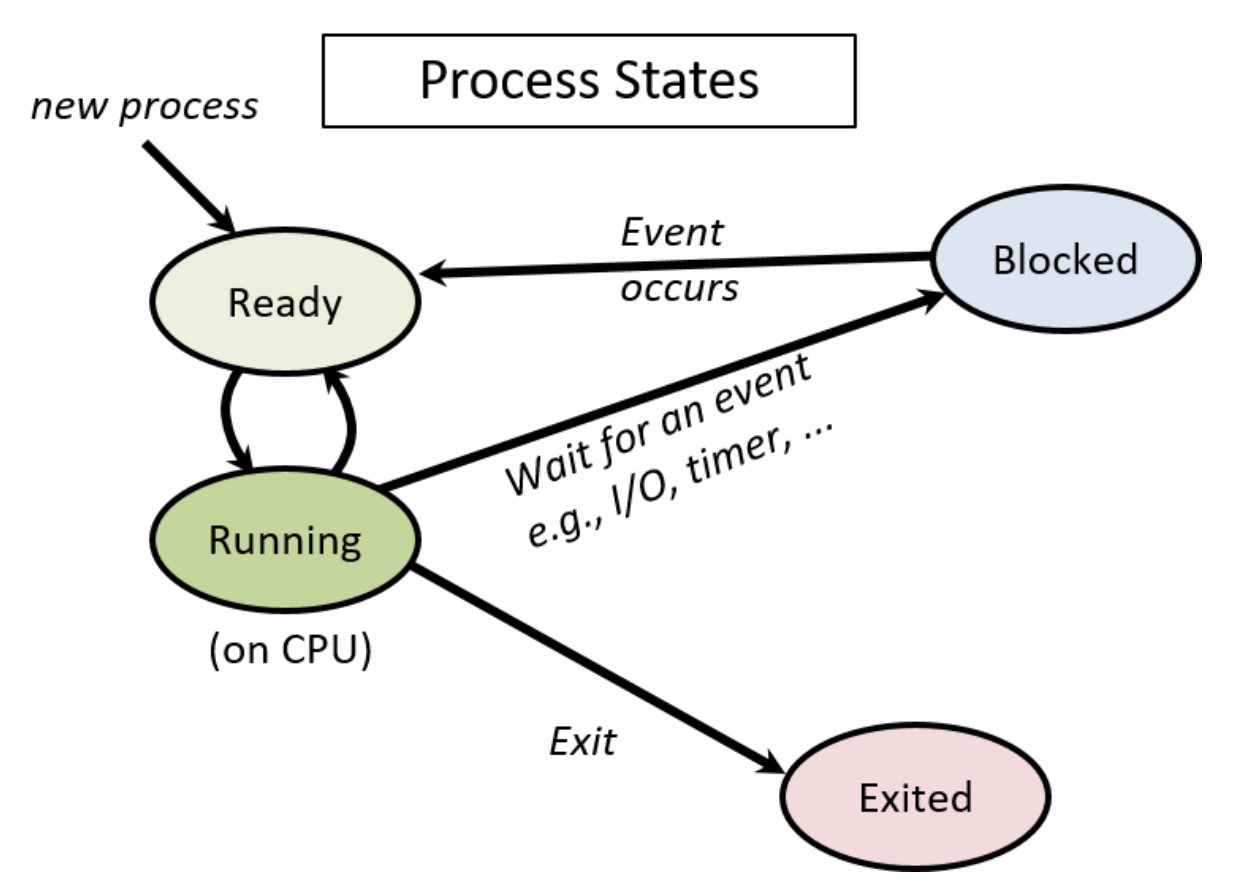
\includegraphics[width=\columnwidth]{images/process-states}
\end{frame}

\begin{frame}{Placeholder}
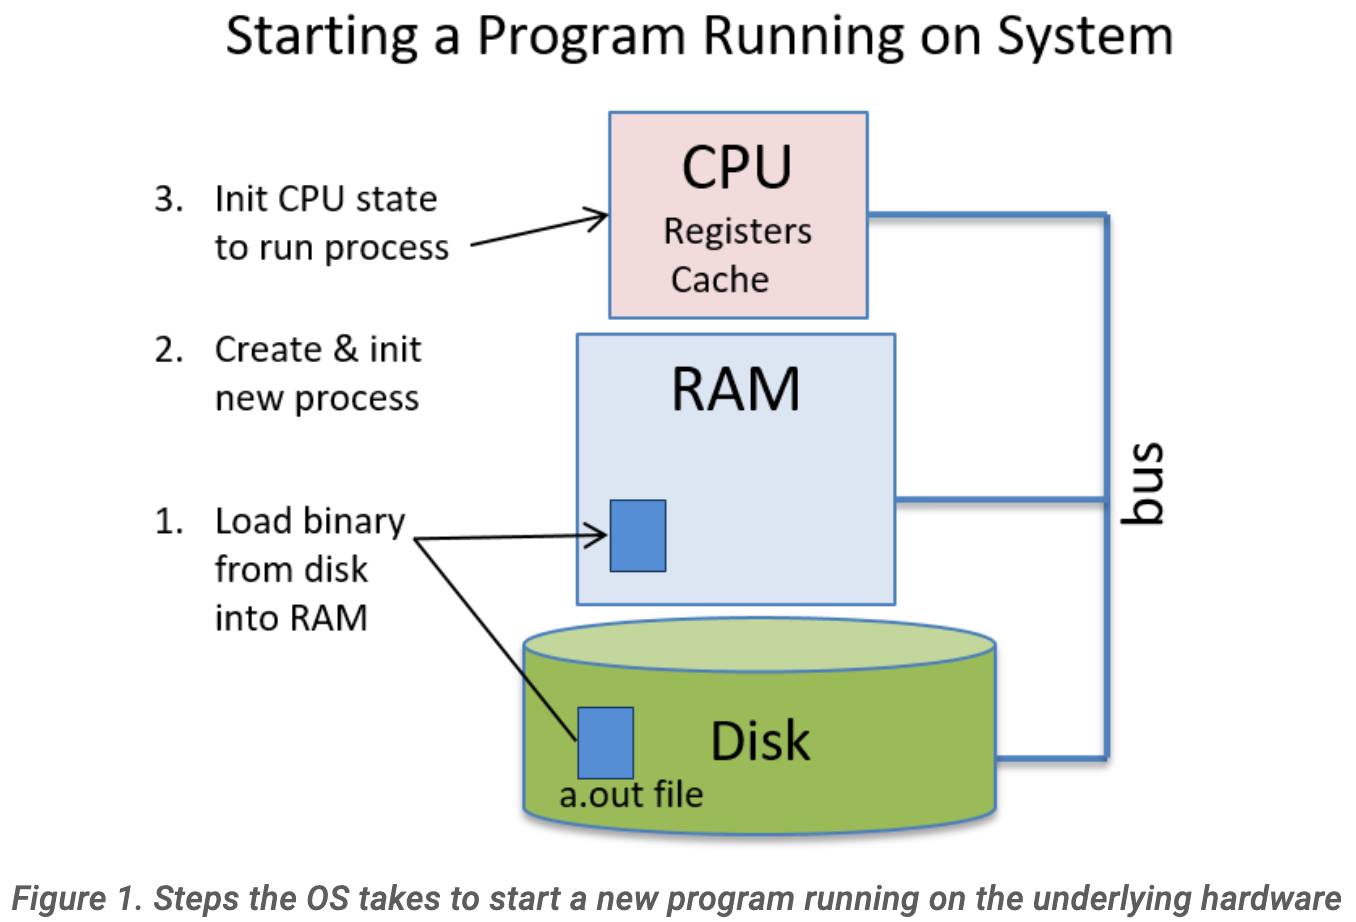
\includegraphics[width=\columnwidth]{images/starting-a-program}
\end{frame}

\begin{frame}{Placeholder}
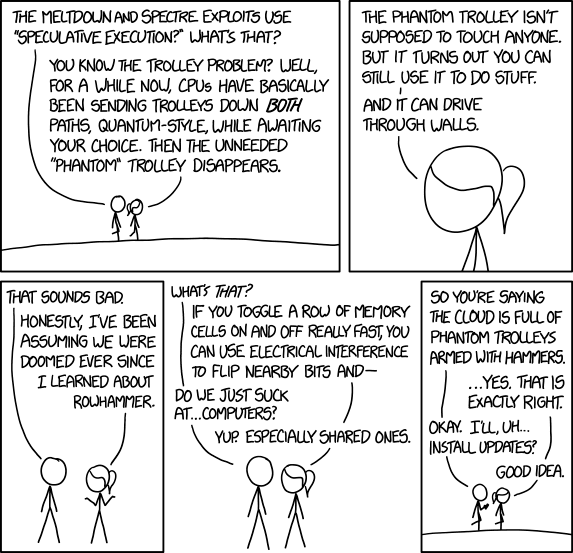
\includegraphics[width=\columnwidth]{images/xkcd-meltdown}
\end{frame}

\begin{frame}{Placeholder}
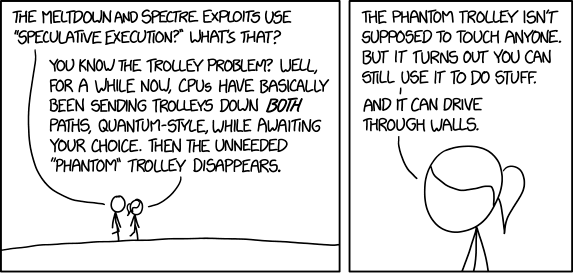
\includegraphics[width=\columnwidth]{images/xkcd-meltdown-cropped}
\end{frame}




\Subsection{The Operating System}


% what is the OS?

% OS kernel

% device interface - allows devices to talk to the kernel

% system call interface - OS allows users to talk to the kernel

% running a program




% vectored events - interrupts and exceptions (fault, trap, abort) - intel x86 terminology

% Per April 2016 version of the Intel Software Developer Manual

% vectored events cause the processor jump to an interrupt handler
% it saves as much context as it can, so execution can later resume

% exceptions/interrupts have an ID (called a vector) that determines which handler

% interrupts are from hardware signals. external devices

% exceptions are from the execution of a program. divide by zero, illegal memory access, page fault

% example: page fault
% try to access something in memory, but it's been swapped out. suspend execution to load it

% trap - program can resume after the instruction that triggered it. example: divide by zero
% fault - program can reattempt the instruction that triggered it. example: page fault. try to access something from memory, but it's been swapped. suspend execution, load it, then try again
% abort - unable to pinpoint the failure. not recoverable. example: hardware failures, corrupted data

% trap is like a precursor to try/catch

% you can also do intentional traps to pass control to the kernel mode. example: file io
% program makes a system call, which the processor turns into a trap

% https://stackoverflow.com/questions/3149175/what-is-the-difference-between-trap-and-interrupt







% interrupts
% computer is idle until an interrupt wakes it up
% example system calls
% File I/O: open, read, write, close
% Process Management: fork, execve, exit
% Memory Management: mmap
% Networking: socket, connect, send, recv

% traps. another word for interrupt? comes from the opposite direction?

% bash system calls
% c system calls

% execution modes. user mode, kernel mode
% address space (OS is mapped into every space)

% meltdown attack


% process hierarchy. fork, child, parent


\Subsection{Threads, Processes, and Cores}






% multiprogramming. switching back and forth fast
% processes
% context switching


% multicore processors
% GPUs - fewer transistors, simpler instruction set
% memory wall - can't keep up with CPU speed increases
% power wall - can't dissipate heat fast enough
% threads. running on different cores, same memory
% wall time vs CPU time


% multithreading - one program using multiple cores. shared memory
% multiprocessing - different processes. possible to split one program into multiple processes (eg supercomputer weather models) but generally not. communication between processes is a lot of work





